\documentclass{beamer}

\usepackage[utf8]{inputenc}
\usepackage[spanish]{babel}
\usepackage{times}
\usepackage{graphicx}
\usepackage{amsmath}
\usepackage{amsthm}
\usepackage{amssymb}

\spanishdecimal{.}

\mode<presentation> {
  \usetheme{Madrid}
  \setbeamercovered{transparent}
}

\title[Redes neuronales] %
{¿Que son las redes neuronales? \\Una introducción informal}

\author[Waissman]{Julio Waissman Vilanova}

\institute[Botón Rojo] %
{Departamento de Matem\'aticas\\
  \textbf{Universidad de Sonora}\\
  para \textbf{Botón Rojo}
}

\date{}

\subject{Neural Network}

\begin{document}


\begin{frame}
  \titlepage
\end{frame}

\begin{frame}
  \frametitle{Plan de la presentación}
  \tableofcontents
  %  % You might wish to add the option [pausesections]
\end{frame}

\section{Motivación}

\begin{frame}
  \frametitle{¿Para que estudiar las redes neuronales?}
  \begin{description}
  \item[Para entender como funciona el cerebro].\\
    El cerebro es una cosa bastante complicada, con partes, que si uno las
    empieza a manipular, el propietario muere generalmente. Por eso los
    métdos de simulación computacional son muy importantes.
    
  \item[Para entender un tipo de computo paralelo].\\  Computo paralelo
    basado en la aplicación masiva de operaciones simples. .
    
  \item[\alert{Para resolver problemas prácticos usando aprendizaje}].\\
    A pesar que las redes neuronales no son un modelo preciso del
    cerebro, se pueden utilizar para resolver una gran cantidad de
    problemas prácticos.
  \end{description}
  
\end{frame}

\begin{frame}
  \frametitle{Estructura de una neurona}
  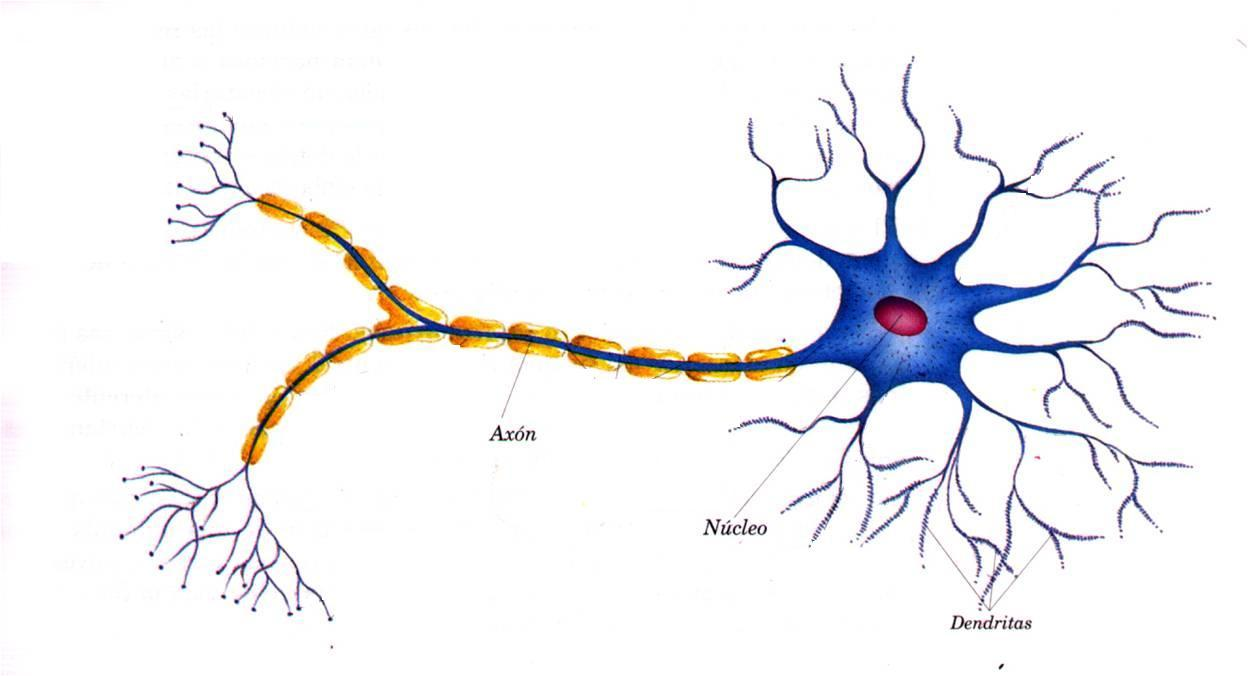
\includegraphics[width=\textwidth]{neurona.jpg}
\end{frame}

\begin{frame}
  \frametitle{Sinapsis}
  \begin{itemize}
  \item Cuando un impulso electrico viaja a través de un axón a una sinapsis, se transmite
    a través de un líquiso neurotransmisor.
  \item El impulso se transmite por difusión a las neuronas receptoras.
  \item La efectividad de las sinapsis puede ser cambiada (peso sináptico).
  \item La sinápisi es lenta, pero usa muy poca energía, y se adapta a partir de señales disponibles localmente.
  \end{itemize}
\end{frame}

\begin{frame}
  \frametitle{¿Como funciona el cerebro?}
  \begin{itemize}
  \item Solo unas pocas neuronas se conectan con receptores o actuadores.
  \item Cada neurona recibe estimulos de otras neuronas.
  \item El efecto de cada entrada de otra neurona es controlado por
    un peso sináptico.
  \item El peso sináptico se adapta de forma que la red en forma global
    aprende a realizar operaciones útiles.
  \item Tenemos aproximadamente $10^11$ neuronas, cada una con $10^4$ pesos sinápticos.
  \end{itemize}
\end{frame}

\begin{frame}
  \frametitle{Modularidad del cerebro}
  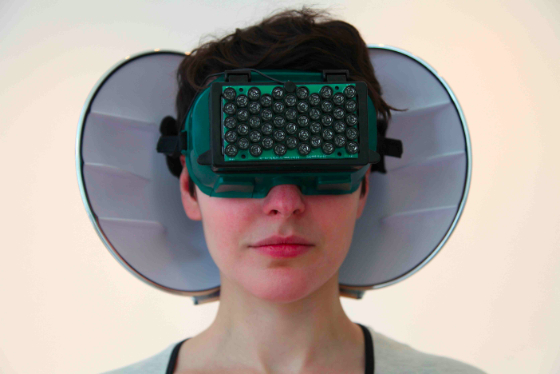
\includegraphics[width=0.9\textwidth]{echo.jpg}  
\end{frame}

\begin{frame}
  \frametitle{Modularidad del cerebro}
  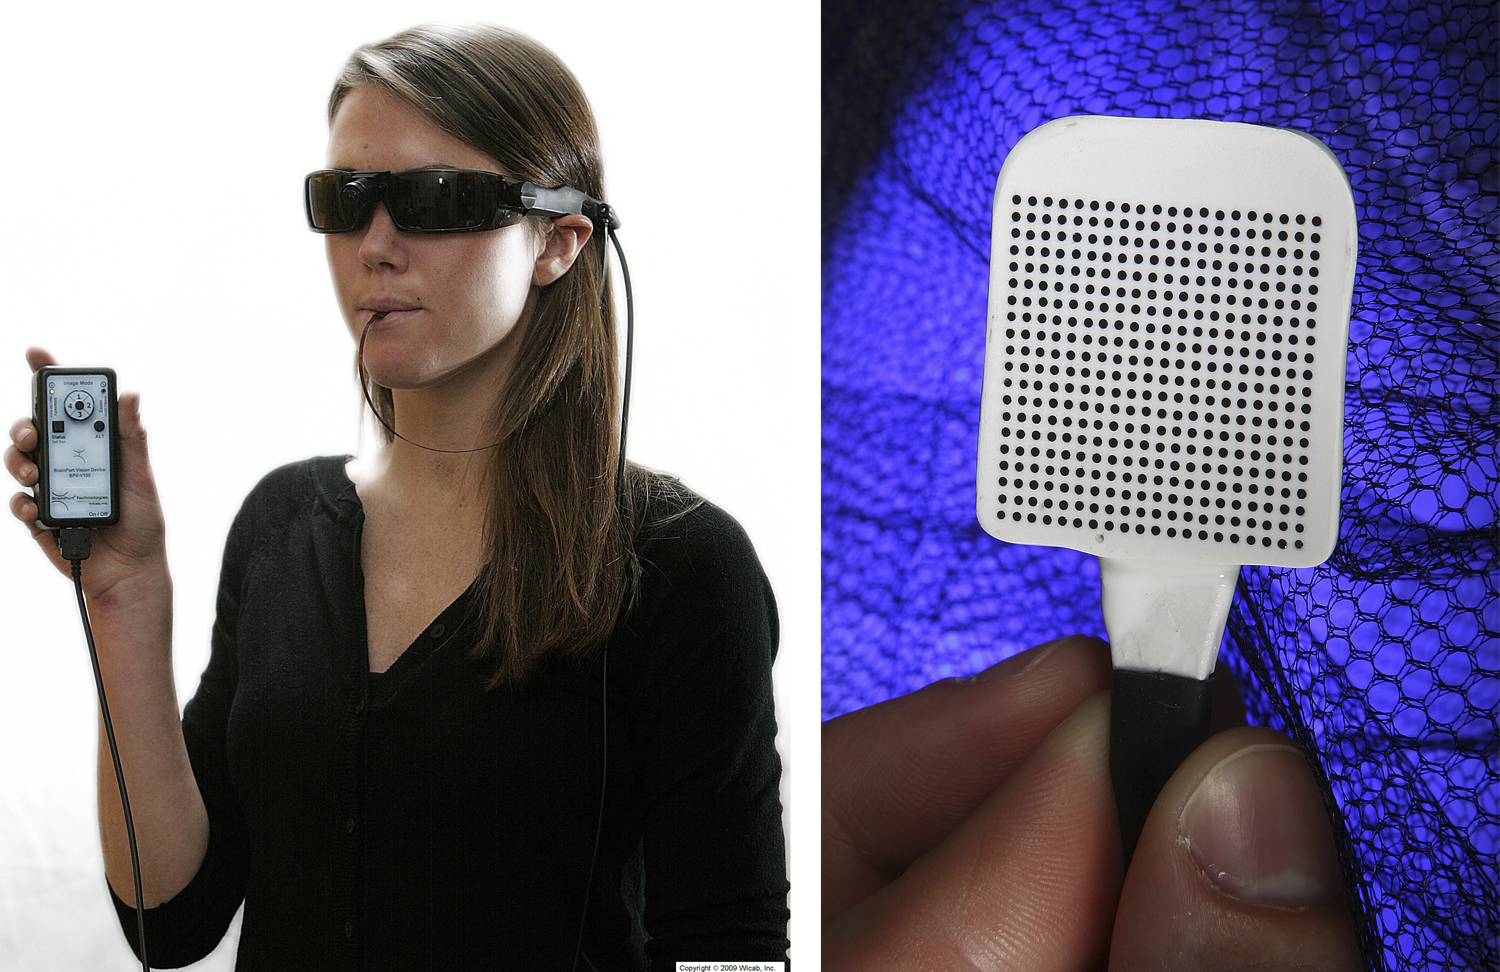
\includegraphics[width=\textwidth]{ver_lengua.jpg}  
\end{frame}



\section{Modelos simples de una neurona}


\section{Un ejemplo simple de aprendizaje}

\section{Tipos de arquitecturas principales}


\section{El perceptrón}



\end{document}

